% Created 2022-09-08 Thu 18:47
% Intended LaTeX compiler: pdflatex
\documentclass[11pt]{article}
\usepackage[utf8]{inputenc}
\usepackage[T1]{fontenc}
\usepackage{graphicx}
\usepackage{longtable}
\usepackage{wrapfig}
\usepackage{rotating}
\usepackage[normalem]{ulem}
\usepackage{amsmath}
\usepackage{amssymb}
\usepackage{capt-of}
\usepackage{hyperref}
\author{Shayan Naqvi}
\date{\today}
\title{Electricity}
\hypersetup{
 pdfauthor={Shayan Naqvi},
 pdftitle={Electricity},
 pdfkeywords={},
 pdfsubject={},
 pdfcreator={Emacs 28.1 (Org mode 9.6)}, 
 pdflang={English}}
\begin{document}

\maketitle
\tableofcontents

\section{Charges}
\label{sec:org2bb7fd4}
The charge of a particle affects its properties.
\begin{itemize}
\item Like charges (positive <-> positive, negative <-> negative) repel.
\item Opposite charges (positive <-> negative) attract.
\item Neutral charges attract with positive/negative charges.
\begin{itemize}
\item Neutrons carry both positive and negative charges; if it comes with close proximity with a charged object, the corresponding charges in the neutron will attract and repel.
\end{itemize}
\end{itemize}
\section{Electric fields}
\label{sec:orge397806}
A region or space around a unit positive charge where it experiences an electrostatic force is known as an electric field.
\begin{center}
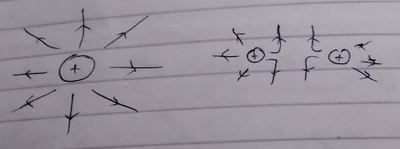
\includegraphics[width=.9\linewidth]{/home/shayan/Documents/org/notes/school/O3/physics/electricity/fig1.png}
\end{center}
\begin{center}
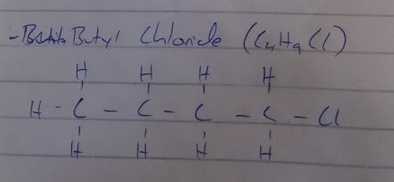
\includegraphics[width=.9\linewidth]{/home/shayan/Documents/org/notes/school/O3/physics/electricity/fig2.png}
\end{center}
\begin{figure}[htbp]
\centering
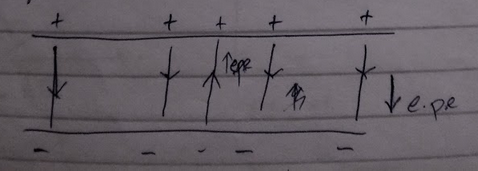
\includegraphics[width=.9\linewidth]{/home/shayan/Documents/org/notes/school/O3/physics/electricity/fig3.png}
\caption{(Uniform field (uniform strength))}
\end{figure}
\begin{itemize}
\item The proximity of the field lines of an electric field determine how strong the field is. The closer the proximity, the stronger the field; the farther the proximity, the weaker the field.
\end{itemize}
\end{document}
